% !TEX encoding = UTF-8
% !TEX TS-program = pdflatex
% !TEX root = ../tesi.tex

%**************************************************************
\chapter{Progettazione}
\label{cap:progettazione}
%**************************************************************

\intro{Questo capitolo illustra le motivazioni alla base delle scelte progettuali adottate nello sviluppo del prototipo da me realizzato durante l'esperienza di stage.}\\ %TODO oppure illustra lo stato dell'applicazione

\section{Architettura preesistente}
Trattandosi di una reimplementazione di una funzionalità preesistente, il primo ostacolo è stato quello di capire come dovesse integrarsi con il resto dell'architettura con cui avrei dovuto interagire, per questo motivo la prima settimana di stage è stata dedicata quasi esclusivamente alla conoscenza dell'ambiente e delle componenti. \\
\subsection{Visione generale}

\begin{figure}[h]
	\centering
	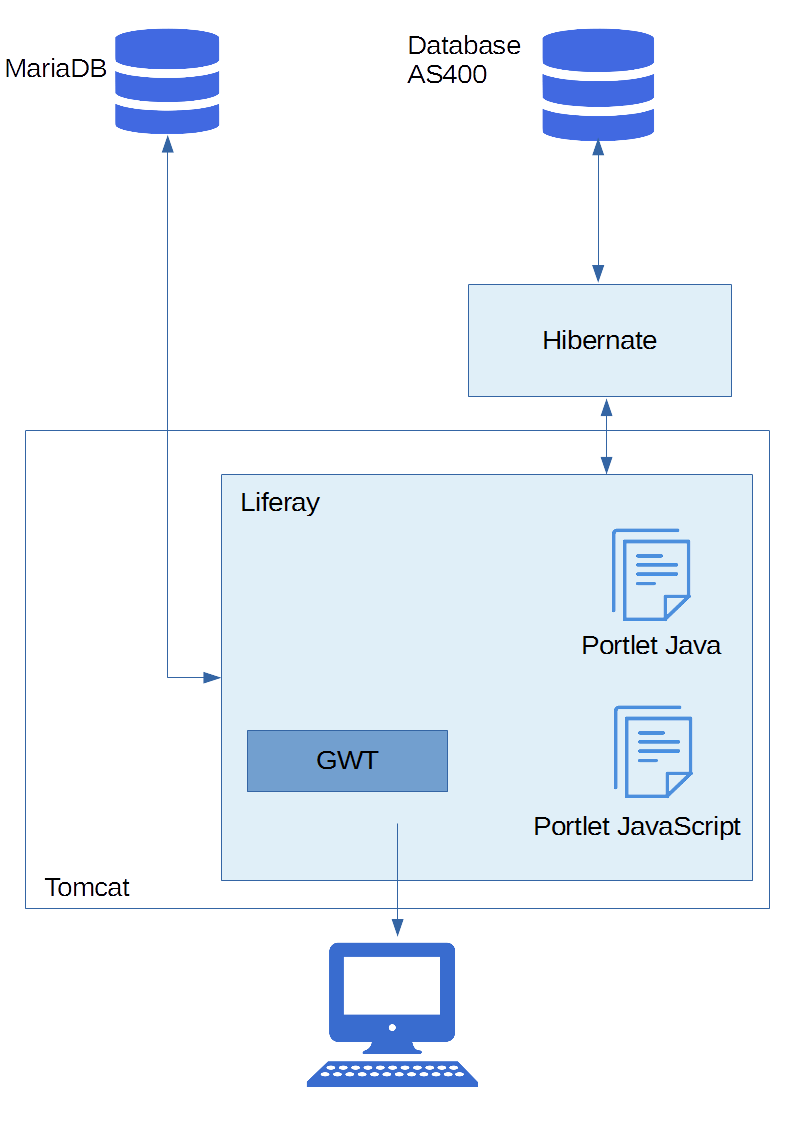
\includegraphics[height = 15 cm]{schema-generale}
	\caption{Schema generale di interconnessione tra le componenti}
	\label{schema-generale}
\end{figure}
la figura \ref{schema-generale} illustra, ad alto livello, le relazioni che intercorrono tra le varie tecnologie utilizzate dal software JGalileo CRM.\\
Partendo dalle basi di dati fino ad arrivare all'interfaccia utente, l'architettura del sistema si snoda in questo modo:\\
Entrambe le basi di dati, sia quella contenuta nel database del sistema operativo AS400 che quella contenuta sul server, si interfacciano con il Framework Hibernate per creare delle classi, equivalenti alle tabelle del database, con cui permettere l'interazione.
\subsubsection{Funzionamento di Hibernate} %TODO ORM
Come avviene la conversione delle tabelle in classi Java?\\
\begin{figure}[h]
	\centering
	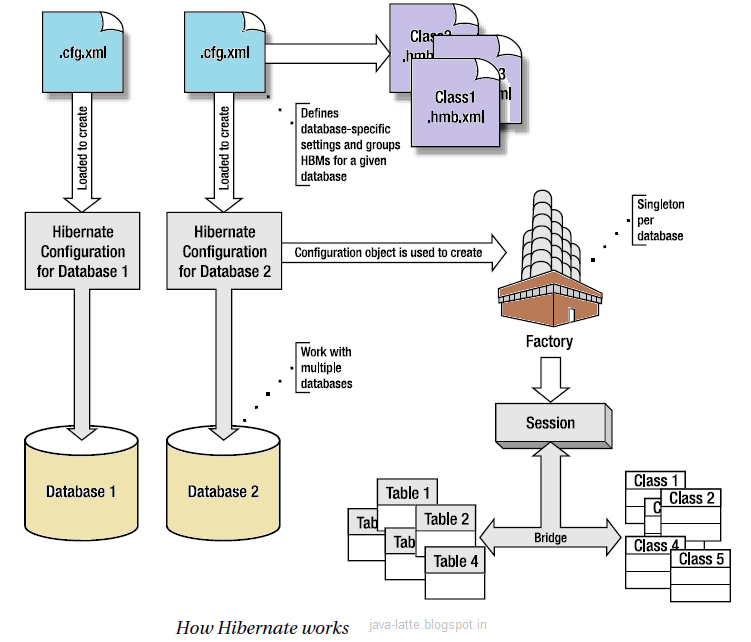
\includegraphics[height = 5 cm]{hibernate_works}
	\caption{Schema del funzionamento di Hibernate}
	\label{schema-generale}
\end{figure}
 Hibernate deve conoscere la configurazione del database e per farlo necessita di un file, estesi generalmente in \textbf{.cfg.xml}. Al framework è inoltre indispensabile fornire dei files di mapping, uno per ogni tabella e generalmente estesi con i suffissi \textbf{.hmb.xml}, che contengono le informazioni riguardanti le colonne della singola tabella da trasformare in un oggetto Java.\\
Questi files vengono poi utilizzati per creare una \emph{SessionFactory} globale e thread-safe che funge da \emph{gateway} per l'interrogazione del database.